

\begin{frame}{Transferring the human power-law to humanoid robots}
\framesubtitle{
  \textcolor{green!30!black!80}
  {
    (K. Matan, BioRob 2016)
  }
}
  \begin{itemize}
    \item Observation : Human moves according to the two-third power-law\\
    \begin{center}
    \tikz[baseline]{\node[fill=txtcolor3,anchor=base]{$ v $};} =
    \tikz[baseline]{\node[fill=blue!50,anchor=base]{$ \gamma $};}
    \tikz[baseline]{\node[fill=green!50,anchor=base]{$ \kappa $};}
    \textsuperscript{\tikz[baseline]{\node[fill=red!50,anchor=base]{$-\beta$};}}
    \end{center}
    \vspace*{-0.5cm}
    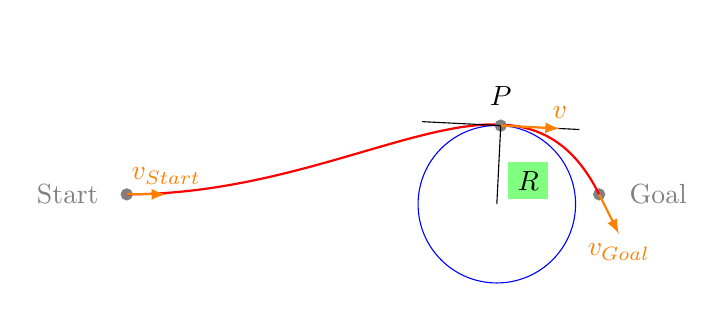
\begin{tikzpicture}
    \node (zero) at (0,0) {};
    \filldraw [gray] ([xshift=-3cm,yshift=-2cm] zero) circle (2pt) + (6,0) circle (2pt);
    \node[color=gray] at ([xshift=-3.75cm,yshift=-2cm] zero) {Start};
    \node[color=gray] at ([xshift=3.75cm,yshift=-2cm] zero) {Goal};
    
    % Trajectory
    \draw[thick,color=red]
    (-3,-2) .. controls +(3,0) and +(-1,2) .. +(6,0);

      % Point in gray
      \filldraw [gray] ([xshift=1.75cm,yshift=-1.1262cm] zero) circle (2pt);
      % Name of the point: P
      \node at ([xshift=1.75cm,yshift=-0.75cm]zero) {$P$};


        % Osculting circle
        \draw[color=blue] (1.7,-2.125) circle (1cm);
        % Drawig Ray to the plot 
        \draw (1.7,-2.125) -- (1.75,-1.1262);
        % Ray label
        \node [fill=green!50] at (2.1,-1.8262) {$R$};
        % Tangent vector to the osculting circle along the trajectory (velocity vector)
        \draw (0.7512,-1.0762) -- (2.7488,-1.1762);

    % Speed
      \draw[-latex,thick,color=orange] (1.75,-1.1262) -- (2.4991,-1.1637)
      node[above] {$v$};

    \draw[-latex,thick,color=orange] (-3,-2) -- (-2.5,-2)
    node[above]{$v_{Start}$};
    
    \draw[-latex,thick,color=orange] (3.0,-2) -- (3.25,-2.5)
    node[below]{$v_{Goal}$};
\end{tikzpicture}
    \item Does this two third power law help humanoid robots to walk?
  \end{itemize}
\end{frame}

\begin{frame}{Drift compensation}
\vspace*{-0.8cm}  
  \begin{center}
    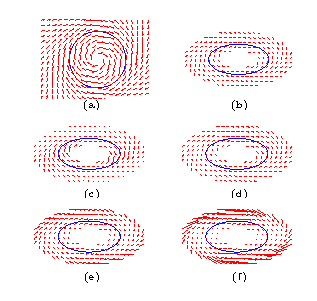
\includegraphics[height = 5.0cm]{two_third/morphing.pdf}
  \end{center}
  \vspace*{-0.5cm}
  \begin{itemize}
    \item Contracting vector field towards cyclic reference trajectories.
    \item (a) unit cycle oscillator, (b) elliptic morphing
    \item (c) $\rightarrow$ (f) $\beta=\{-\frac{1}{3},0,\frac{1}{3},\frac{2}{3}\}$
  \end{itemize}
\end{frame}

\begin{frame}{Full controller}
  \begin{center}
    \scalebox{0.7}{\begin{tikzpicture}%[show background grid]% every node/.style={draw,outer sep=0pt,thick}]

% SoT
\draw [fill=green,opacity=.2,text opacity=1] (-1.5,2.2) rectangle (13.0,-2.2);
\node at(6,-2.0) {\textcolor{green!20!black!100}{Stack of Tasks}};

% Ellispe Reference
\node[rectangle,minimum width=2cm, minimum height=1cm,draw=blue!70,fill=blue!20] (ellipseref) at (4.0,3.25) {};
\node[ellipse,draw=blue,thick,minimum width=1cm,minimum height=0.5cm] at (ellipseref) {};
\node at ([yshift=-0.8cm]ellipseref) {Reference trajectory};

% Vector Field
\node[rectangle,minimum width=2cm, text width=2cm,minimum height=1cm,draw=blue!70,fill=blue!20,align=center] (vectorfields) at (0.0,0.0) 
{Vector Field\\
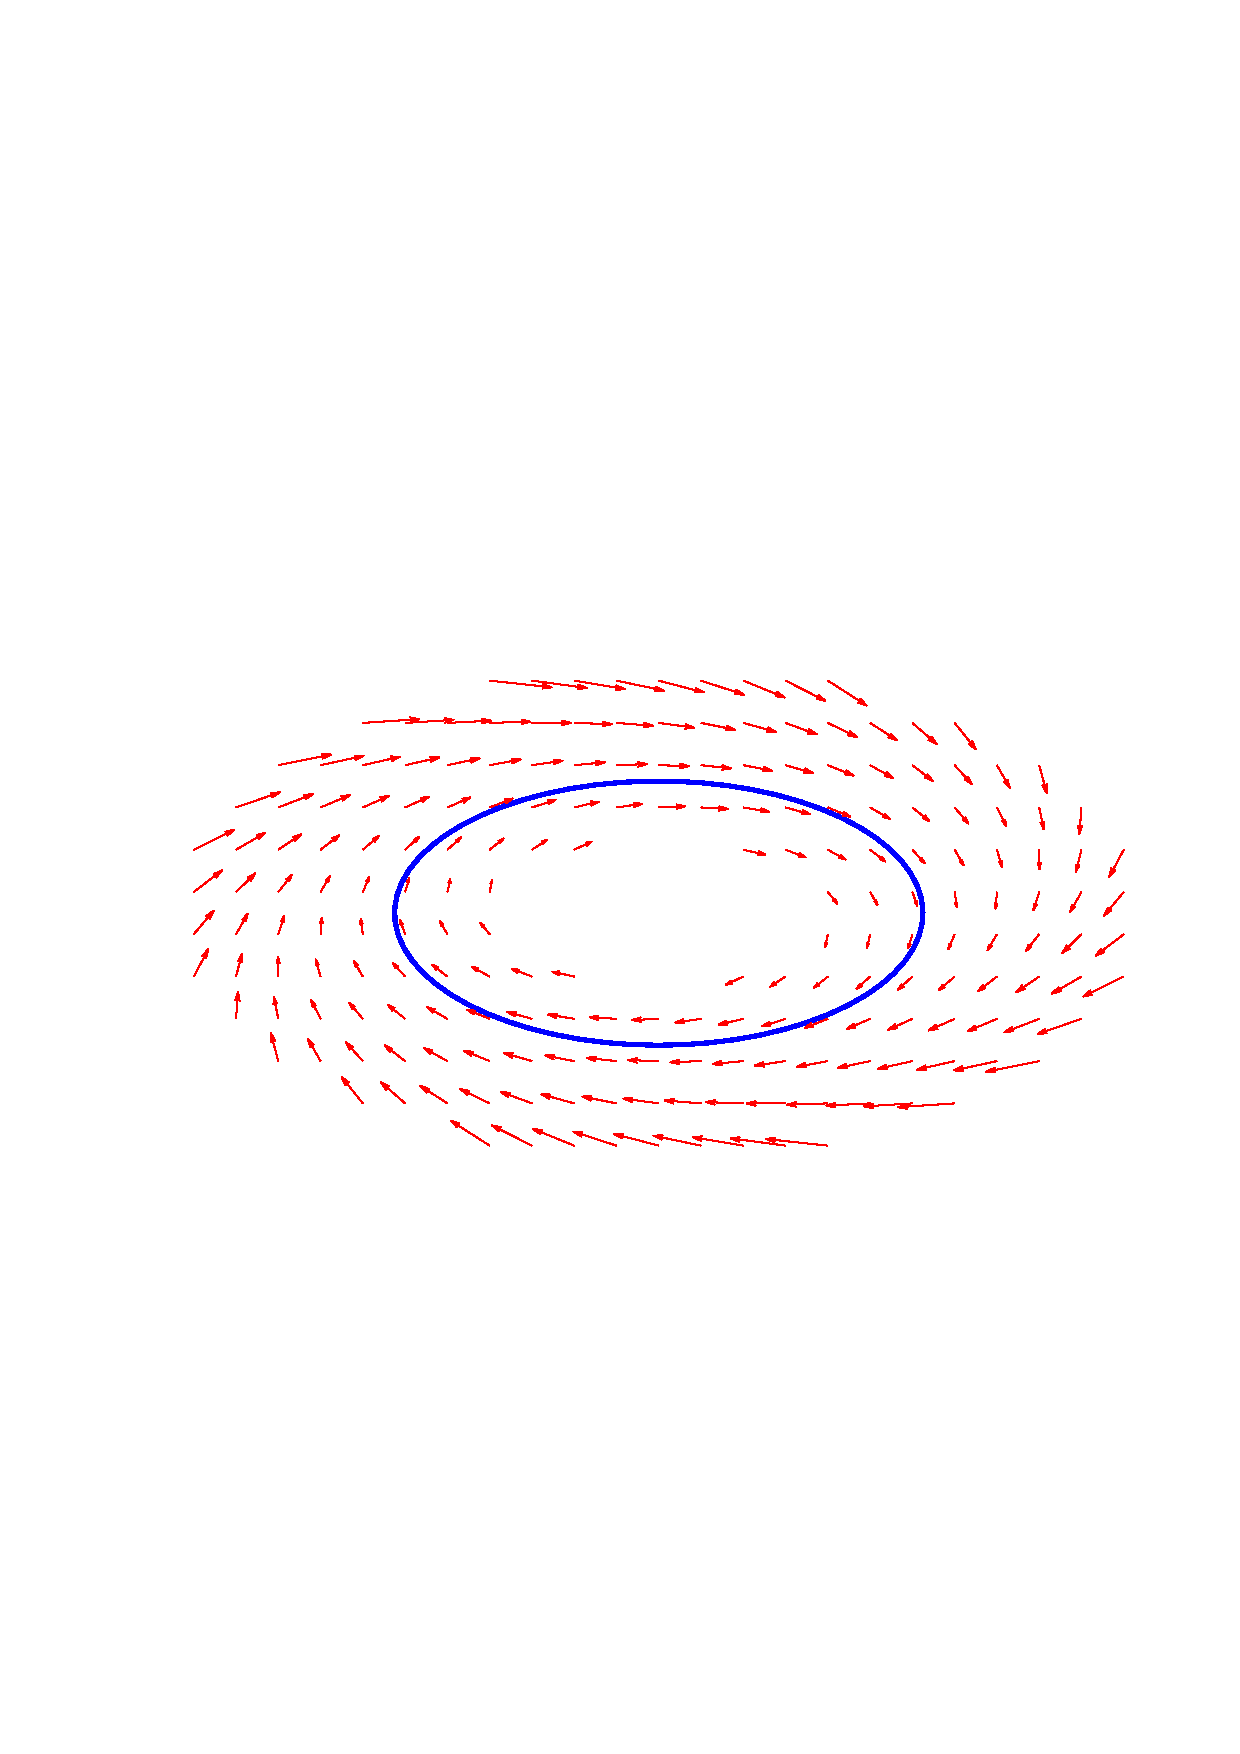
\includegraphics[scale=0.1]{two_third/Fig3e_EllipseBetaThird.pdf}
};
%\node at (0.0,2.5) {$\gamma,\beta$};

% Walking Pattern Generator
\node[rectangle,minimum width=2cm, minimum height=1cm,draw=blue!70,fill=blue!20]  (wpg) at (5.4,1.0) {Walking Pattern Generator};

% Task
\node[rectangle,minimum width=2cm, text width=3cm, align=center, minimum height=1cm,draw=blue!70,fill=blue!20] (ttt) at (11,1.0) 
{  Tasks for\\
   Trajectory\\
   Tracking};

% Solver
\node[rectangle,minimum width=2cm, text width=3cm, align=center, minimum height=1cm,draw=blue!70,fill=blue!20] (qp) at (11,-1.0) 
{ HQP Solver };

% Power Law
\node[rectangle,text width=2cm,align=center,minimum width=2cm, minimum height=1cm,draw=blue!70,fill=blue!20] (powerlaw) at (3.0,-1.0) {Power Law\\$\gamma,\beta$};
\path[->,>=stealth',draw=black] (vectorfields.314)-- node[below] {$\kappa$} (powerlaw.189);
\path[->,>=stealth',draw=black] (powerlaw.170)-- node[above] {$v$} (vectorfields.325);

% Robot
\node[rectangle,minimum width=2cm, minimum height=1cm,draw=blue!70,fill=blue!20] (robot) at (11,-3.5) {Robot};

% Localization
\node[rectangle,minimum width=2cm, minimum height=1cm,draw=blue!70,fill=blue!20] (localization) at (0.0,-3.5) {Localization};

%\path[->,>=stealth',draw=black] (0.0,2.25)-- (vectorfields.90);

% Links
\draw[->,>=stealth',draw=black] (ellipseref.180) -| (vectorfields.90);
\draw[->,>=stealth',draw=black] (vectorfields.42) -- node[above] {${\bf c}^*$} (wpg.180);
\path[->,>=stealth',draw=black] (wpg)-- node[above] {
$\begin{matrix}
{c}_{ref}\\{\bf z}_{ref}\\{\bf LF}_{ref}\\{\bf RF}_{ref}
\end{matrix} $
}(ttt);
\path[->,>=stealth',draw=black] (ttt)-- node[right] {\small Tasks} (qp);
\path[->,>=stealth',draw=black] (qp)-- node[xshift=0.2cm,yshift=-0.2cm,] {${\bf q}$} (robot);
\path[->,>=stealth',draw=black] (robot)-- node[below,font=\small] {Motion capture}(localization);
\path[->,>=stealth',draw=black] (localization)-- node[left] {${\bf w}$}(vectorfields);

\end{tikzpicture}
} \\
  \end{center}
\end{frame}

\begin{frame}{Results}
  \begin{center}
    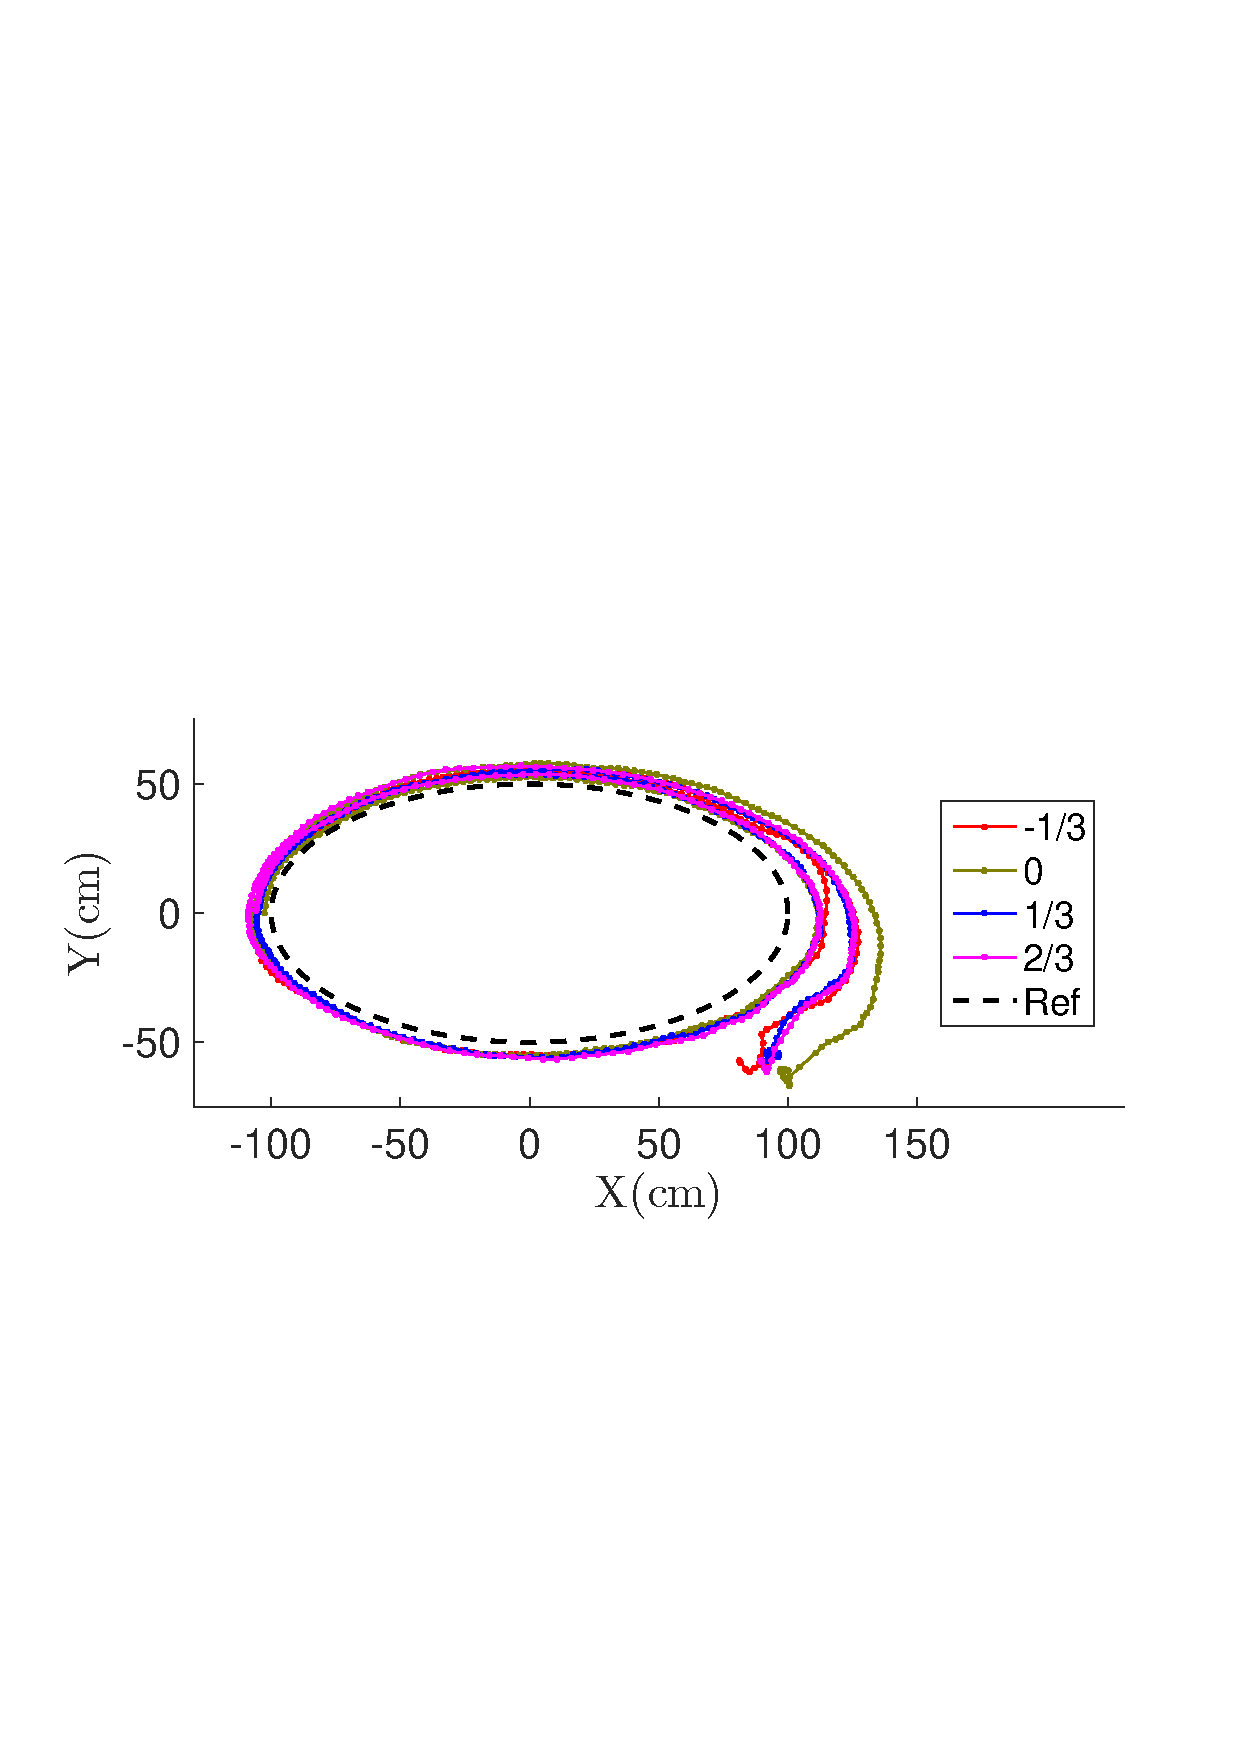
\includegraphics[trim={1.0cm 10.0cm 1.0cm 13.0cm}, clip,height = 3.0cm]
    {two_third/Fig5d_EXPshapesSymmetric.pdf}
    %trim={<left> <lower> <right> <upper>}
    \hfill
    \begin{table}[ht]
    	\centering 
	  \begin{tabular}{| c | c | c | c | c |c |} 
		  \hline 
		  Ref.~$\beta$        & $-\frac{1}{3}$  & $0$      & \textcolor{red}{$\frac{1}{3}$} & $\frac{2}{3}$   \\
		  \hline  
		  Norm     ($m$)        & $1.416$  & $0.950$  & \textcolor{red}{$0.642$} & $1.124$ \\   
		  Orientation ($deg$)   & $76.83$  & $89.60$  & \textcolor{red}{$60.45$} & $77.28$ \\ 
		  Tangential Force ($kN \; s$) & $21.93 $ & $23.54$  & \textcolor{red}{$19.80$} &$21.01$  \\ 
		  \hline 		  
	  \end{tabular}
  \end{table}
  \end{center}
  \blfootnote{(Karklinsky et al. BioRob 2016)}
%  
%  Globally, the     values of the simulated motions reflect the ones of     the reference trajectory 
%
%The position of maximal speed on simulated trajectories is slightly shifted  (delayed)
%
%Unpredictably, for         ,  an oscillatory curvature-dependent speed profile is observed
%
%The controlled motions take more time than the reference movement. The higher     the faster the motion. 
\end{frame}





